% This must be in the first 5 lines to tell arXiv to use pdfLaTeX, which is strongly recommended.
\pdfoutput=1
% In particular, the hyperref package requires pdfLaTeX in order to break URLs across lines.

\documentclass[11pt]{article}

% Remove the "review" option to generate the final version.
\usepackage{ACL2023}
\usepackage{graphicx}
% Standard package includes
\usepackage{times}
\usepackage{latexsym}

% For proper rendering and hyphenation of words containing Latin characters (including in bib files)
\usepackage[T1]{fontenc}
% For Vietnamese characters
% \usepackage[T5]{fontenc}
% See https://www.latex-project.org/help/documentation/encguide.pdf for other character sets

% This assumes your files are encoded as UTF8
\usepackage[utf8]{inputenc}

% This is not strictly necessary, and may be commented out.
% However, it will improve the layout of the manuscript,
% and will typically save some space.
\usepackage{microtype}

% This is also not strictly necessary, and may be commented out.
% However, it will improve the aesthetics of text in
% the typewriter font.
\usepackage{inconsolata}

\usepackage{listings}
\usepackage{xcolor}

\definecolor{codegreen}{rgb}{0,0.6,0}
\definecolor{codegray}{rgb}{0.5,0.5,0.5}
\definecolor{codepurple}{rgb}{0.58,0,0.82}
\definecolor{backcolour}{rgb}{0.95,0.95,0.92}

\lstdefinestyle{mystyle}{
    backgroundcolor=\color{backcolour},   
    commentstyle=\color{codegreen},
    keywordstyle=\color{magenta},
    numberstyle=\tiny\color{codegray},
    stringstyle=\color{codepurple},
    basicstyle=\ttfamily\footnotesize,
    breakatwhitespace=false,         
    breaklines=true,                 
    captionpos=b,                    
    keepspaces=true,                 
    numbers=left,                    
    numbersep=5pt,                  
    showspaces=false,                
    showstringspaces=false,
    showtabs=false,                  
    tabsize=2
}

\lstset{style=mystyle}
% If the title and author information does not fit in the area allocated, uncomment the following
%
%\setlength\titlebox{<dim>}
%
% and set <dim> to something 5cm or larger.

\title{Image Recognition using k-NN}

% Author information can be set in various styles:
% For several authors from the same institution:
% \author{Author 1 \and ... \and Author n \\
%         Address line \\ ... \\ Address line}
% if the names do not fit well on one line use
%         Author 1 \\ {\bf Author 2} \\ ... \\ {\bf Author n} \\
% For authors from different institutions:
% \author{Author 1 \\ Address line \\  ... \\ Address line
%         \And  ... \And
%         Author n \\ Address line \\ ... \\ Address line}
% To start a seperate ``row'' of authors use \AND, as in
% \author{Author 1 \\ Address line \\  ... \\ Address line
%         \AND
%         Author 2 \\ Address line \\ ... \\ Address line \And
%         Author 3 \\ Address line \\ ... \\ Address line}

\author{Zhang Huakang \\
  \texttt{mc35095@um.edu.mo} \\}

\begin{document}
\maketitle
\begin{abstract}
  In this project, we implement a k-NN classifier to recognize the images in CIFAR-10 dataset. We use different image processing methods to preprocess the dataset, and use different distance metrics to test the performance of the classifier. We also implement a k-NN with PCA classifier, SVM and NN, to compare the performance of the k-NN.
\end{abstract}

\section{Introduction}
In this porject, we are going to implement a k-NN classifier to recognize the images. 
The dataset we use is CIFAR-10, which contains 60000 images in 10 classes. 
The images are 32x32 RGB images. We will use the training set to train the classifier and use the test set to test the classifier. 
The classifier will predict the class of the test images and compare the prediction with the ground truth to calculate the accuracy. 

Not only k-NN classifier, we will also implement a k-NN with PCA classifier, SVM, and NN, to compare the performance of the k-NN.

We use Python to implement the project, and the code is available at Github\footnote{\url{https://github.com/BoxMars/CISC704-HW/tree/main/HW1}}

\section{Background}
\subsection{Image Recognition}
Image recognition is the ability of AI to detect objects, places, people, writing and actions in images, which has been a popular topic in the field of computer vision. There are many datasets for image recognition, such as CIFAR-10, CIFAR-100, MNIST, etc. In this project, we will use CIFAR-10 dataset.
\subsection{CIFAR-10}
CIFAR-10\footnote{\url{https://www.cs.toronto.edu/~kriz/cifar.html}} is a dataset of 60000 32x32 color images in 10 classes, with 6000 images per class. 
There are 50000 training images and 10000 test images. The dataset is divided into five training batches and one test batch, each with 10000 images. 
The test batch contains exactly 1000 randomly-selected images from each class. 
The training batches contain the remaining images in random order, but some training batches may contain more images from one class than another. 
Between them, the training batches contain exactly 5000 images from each class. 
\begin{figure}[h]
    \centering
    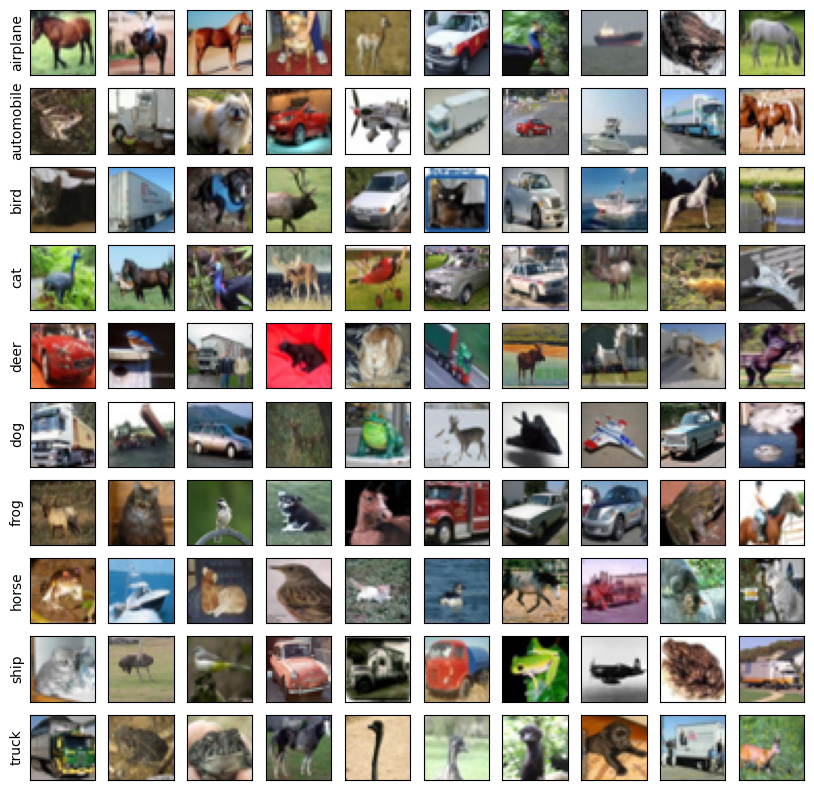
\includegraphics[width=0.5\textwidth]{color.png}
    \caption{CIFAR-10}
    \label{fig:cifar10}
\end{figure}
\subsection{scikit-learn\cite{scikit-learn}}

scikit-learn\footnote{\url{https://scikit-learn.org/stable/}} is a free software machine learning library for the Python programming language. All algorithm used in this project are implemented by scikit-learn.  

But this library has some limitations, such as it does not support GPU which means it is not suitable for large-scale machine learning.

\subsection{cuML}
cuML\footnote{\url{https://docs.rapids.ai/api/cuml/stable/}} cuML is a suite of fast, GPU-accelerated machine learning algorithms designed for data science and analytical tasks whose API mirrors that of scikit-learn. cuML enables data scientists, researchers, and software engineers to run traditional tabular ML tasks on GPUs without going into the details of CUDA programming.

In this project, we use cuML to implement the k-NN classifier, SVM and PCA, which is much faster than scikit-learn.
\section{Method}

\subsection{Nearest Neighbors \& k-Nearest Neighbors}

% different between NN and k-NN
Nearest Neighbors (NN) is a simple algorithm that stores all available cases and classifies new cases based on a similarity measure (e.g., distance functions), 
while k-Nearest Neighbors (k-NN) is a variant of NN, which is a non-parametric method used for classification and regression and is a voting algorithm based on the k closest neighbors, 
when $k=1$, it is the NN algorithm.

\subsection{Principal Component Analysis}
Principal component analysis (PCA) is a statistical procedure that uses an orthogonal transformation to convert a set of observations of possibly correlated variables into a set of values of linearly uncorrelated variables called principal components. The number of principal components is less than or equal to the number of original variables. This transformation is defined in such a way that the first principal component has the largest possible variance (that is, accounts for as much of the variability in the data as possible), and each succeeding component in turn has the highest variance possible under the constraint that it is orthogonal to the preceding components. The resulting vectors are an uncorrelated orthogonal basis set. PCA is sensitive to the relative scaling of the original variables.

\subsection{Support Vector Machine}

Support Vector Machine (SVM) is a supervised machine learning algorithm that can be used for both classification or regression challenges. However, it is mostly used in classification problems. In the SVM algorithm, we plot each data item as a point in n-dimensional space (where n is the number of features you have) with the value of each feature being the value of a particular coordinate. Then, we perform classification by finding the hyper-plane that differentiates the two classes very well.

\subsection{Image Processing}
The images in CIFAR-10 are 32x32 RGB images, which means each image has 32x32x3=3072 features. When we use k-NN to classify the images, the dimension of the feature space is too large, which will cause the curse of dimensionality. So we need to reduce the dimension of the feature space.

\subsection{Gary Scale}
The first method we use is to convert the RGB images to gray scale images. The gray scale images only have one channel, which means the dimension of the feature space is reduced from 3072 to 1024.
Fig 2 shows the gray scale images of CIFAR-10.
\begin{figure}[h]
    \centering
    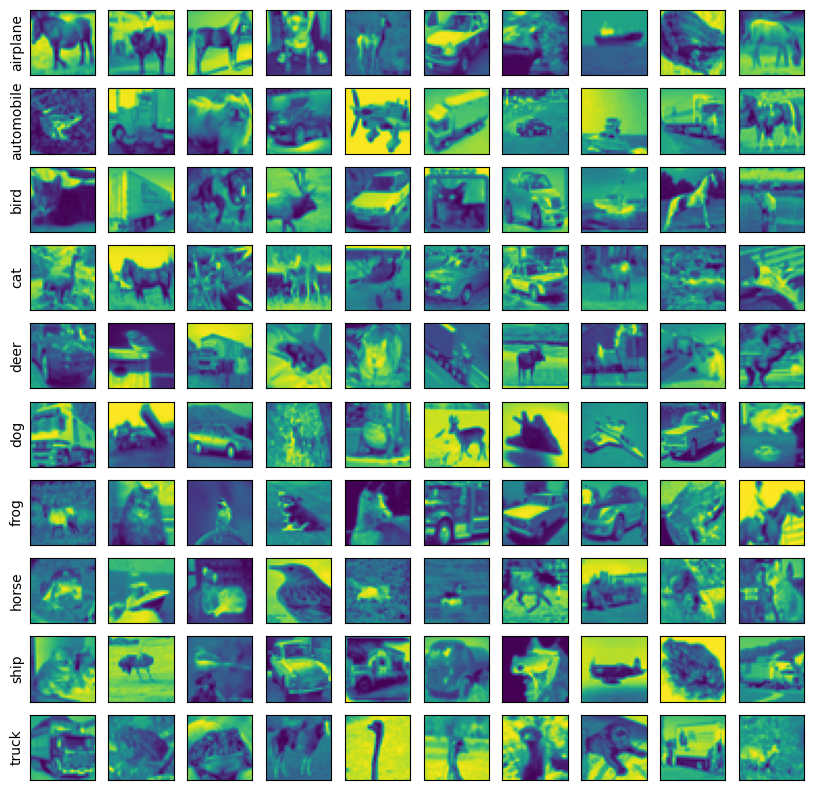
\includegraphics[width=0.5\textwidth]{gray.png}
    \caption{Gray Scale}
    \label{fig:gray}
\end{figure}
\subsection{Binary Image}

The second method we use is to convert the gray images to binary images. The binary images only have two values, 0 and 1.
Fig 3 shows the binary images of CIFAR-10.
\begin{figure}[h]
    \centering
    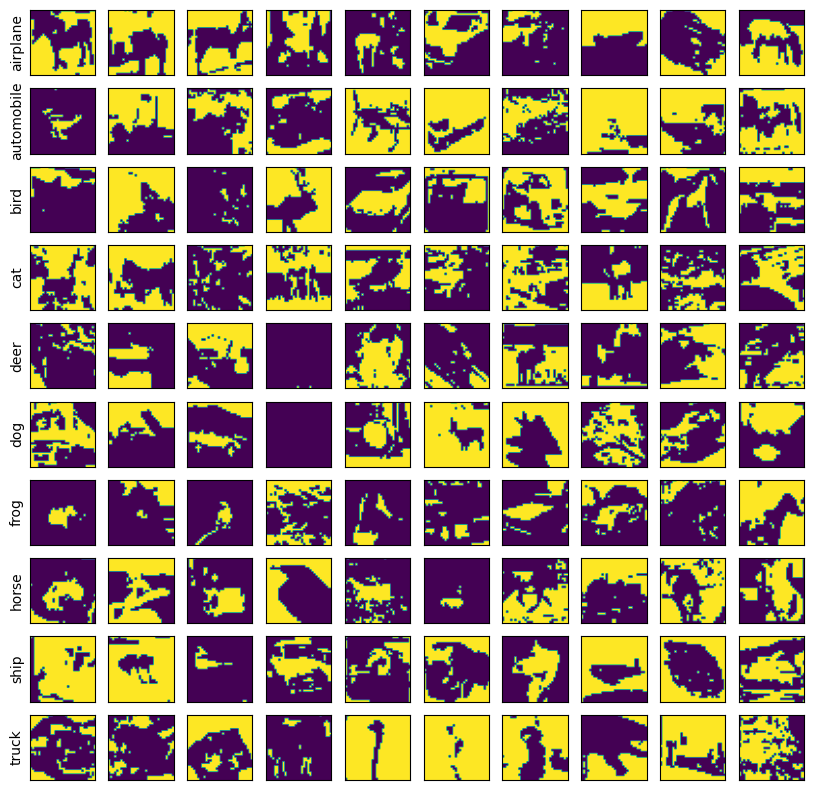
\includegraphics[width=0.5\textwidth]{binary.png}
    \caption{Binary Image}
    \label{fig:binary}
\end{figure}

\subsection{HSV}
The third method we use is to convert the RGB images to HSV images. HSV is a color model that describes colors (hue or tint) in terms of their shade (saturation or amount of gray) and their brightness value. The HSV images have three channels.
Fig 4 shows the HSV images of CIFAR-10.
\begin{figure}[h]
    \centering
    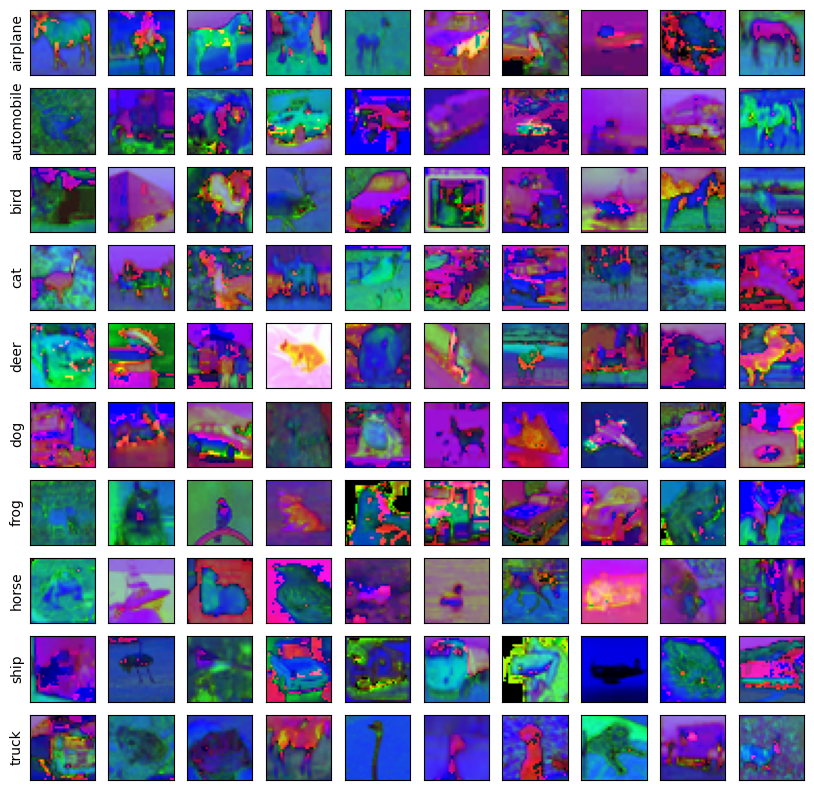
\includegraphics[width=0.5\textwidth]{hsv.png}
    \caption{HSV}
    \label{fig:hsv}
\end{figure}

\subsection{Edge Detection}
In this project, we use \verb|skimage.feature.canny|
\footnote{\url{https://scikit-image.org/docs/dev/api/skimage.feature.html#skimage.feature.canny}}
to detect the edges of the images. The edge detection algorithm will return a binary image.
Fig 5 shows the edge images of CIFAR-10.
\begin{figure}[h]
    \centering
    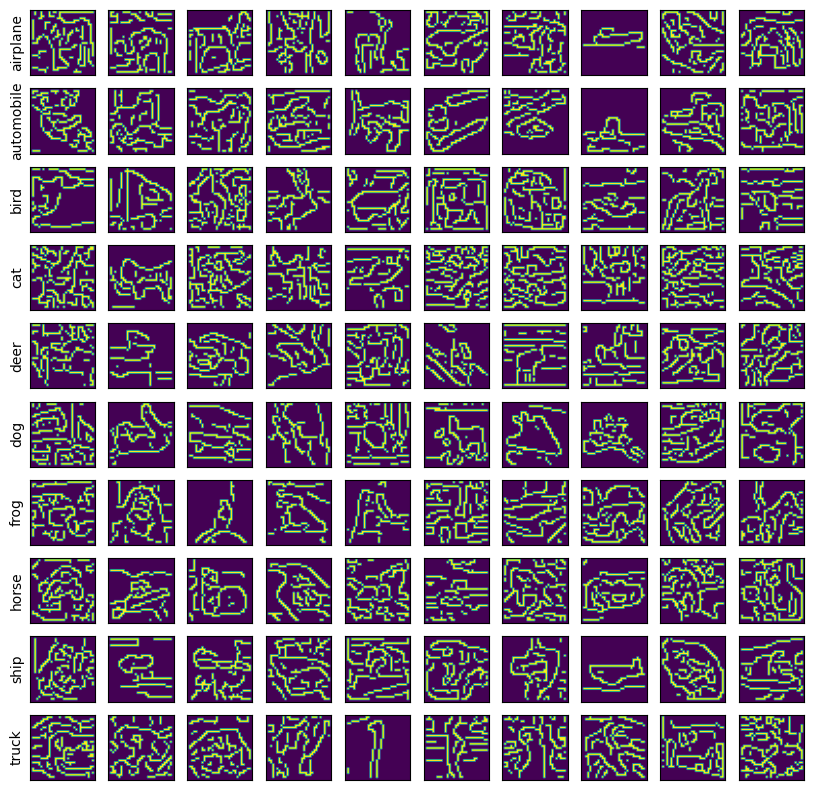
\includegraphics[width=0.5\textwidth]{canny.png}
    \caption{Edge Detection}
    \label{fig:edge}
\end{figure}

\subsection{Histogram of Oriented Gradients}
Histogram of Oriented Gradients (HOG) is a feature descriptor used in computer vision and image processing for the purpose of object detection. 
The technique counts occurrences of gradient orientation in localized portions of an image. 
This method is similar to that of canny, but differs in that it is computed on a dense grid of uniformly spaced cells and uses overlapping local contrast normalization for improved accuracy.
Fig 6 shows the HOG images of CIFAR-10.

\begin{figure}[h]
    \centering
    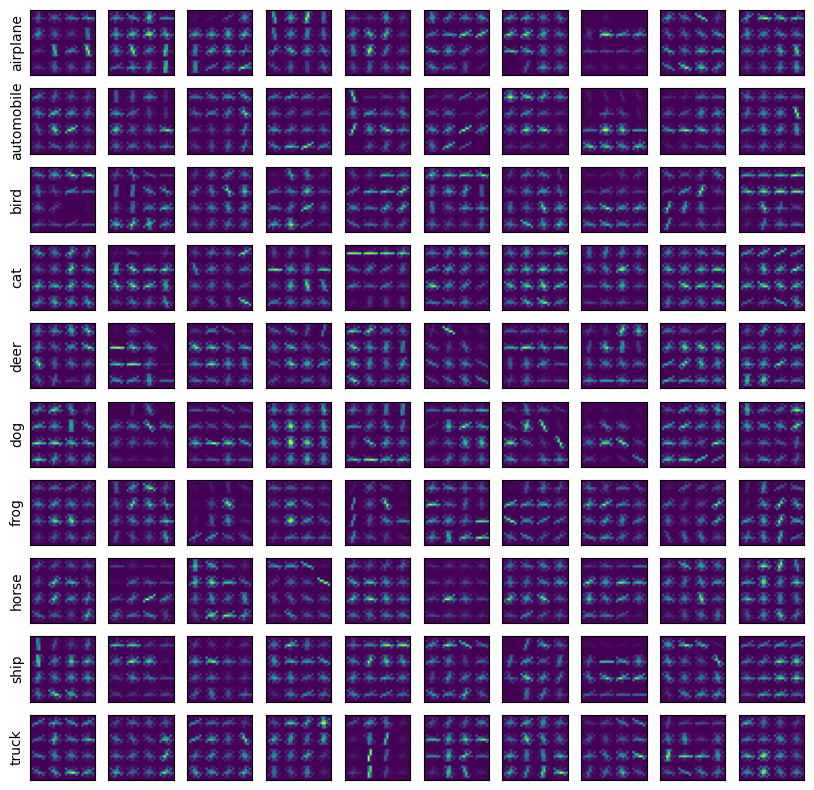
\includegraphics[width=0.5\textwidth]{hog.png}
    \caption{Histogram of Oriented Gradients}
    \label{fig:hog}
\end{figure}
\section{Experiments}
\subsection{Download Dataset}
CIFAR-10 dataset is available at \url{https://www.cs.toronto.edu/~kriz/cifar.html}. We can download the dataset from the website using \verb|requests| python library and unzip it using
\verb|tarfile| library. 

The data file of CIFAR-10 is a binary file, which can be read using \verb|pickle| library. 

\subsection{Preprocess Dataset}

We use the APIs provided by scikit-learn to preprocess the dataset. The first step is to convert the RGB images to gray scale images, binary images, HSV images, edge images and HOG images.

The second step is shuffle the dataset bescause the dataset is ordered by class and wo noticed the accuracy of unshuffled dataset is higher than shuffled dataset. 
Before shuffling the dataset, we need to convert the dataset to numpy array, and set the random seed to 0 to make sure the result is reproducible.

\subsection{k-NN Classifier on GPU}
We use cuML to implement the k-NN classifier on GPU. 
\begin{lstlisting}[language=Python, caption={k-NN Classifier on GPU}]
from cuml.neighbors import NearestNeighbors

classifiers = [
    ('NN with L1 distance', NearestNeighbors(n_neighbors=1, verbose=True, metric='l1')),
    ('NN with L2 distance', NearestNeighbors(n_neighbors=1, verbose=True, metric='l2')),
    ('NN with cosine', NearestNeighbors(n_neighbors=1, verbose=True, metric='cosine')),
]
\end{lstlisting}

When \verb|n_neighbors| is $1$, it is the NN classifier. We use three different distance metrics, L1 distance, L2 distance and cosine distance and test the performance of different \verb|n_neighbors| from $1$ to $20$.
The reslut is shown in Fig 7. From the result, we can see that the accuracy of NN with L1 distance is higher than L2 distance and cosine distance, and the image with hog feature has the highest accuracy, and the second is the image with gray scale feature.

The accuracy of the classifier will increase as the number of neighbors increases. 
When the number of neighbors is larger than $5$, the accuracy of the classifier will not increase significantly.

\begin{lstlisting}[language=Python,caption={k-NN Classifier on GPU with different neighbors}]
def predict(classifiers, train_imgs, train_labels, test_imgs):
  train_imgs = train_imgs.reshape((50000, -1))
  test_imgs = test_imgs.reshape((10000, -1))

  # shuffle data
  np.random.seed(0)
  np.random.shuffle(train_imgs)
  np.random.seed(0)
  np.random.shuffle(train_labels)
  np.random.seed(0)
  np.random.shuffle(test_imgs)
  np.random.seed(0)
  np.random.shuffle(test_labels)
  

  # combination of train img and label
  train = np.hstack((train_imgs, train_labels))
  test = np.hstack((test_imgs, test_labels))

  accs={}
  for name, model in classifiers:
      accs[name] = []
      model.fit(train)
      for i in range(1,21):
          distance, indices = model.kneighbors(test, n_neighbors=i, return_distance=True)
      
          pred = train_labels[indices]
          # find the most common label
          pred = np.apply_along_axis(lambda x: np.argmax(np.bincount(x)), axis=1, arr=pred)
          
          pred = pred.reshape((10000, 1))
          acc = accuracy_score(test_labels, pred)
          # print('Accuracy of {} - k: {}: {}'.format(name, i, acc))
          accs[name].append(acc)
  return accs
\end{lstlisting}

\begin{figure}
    \centering
    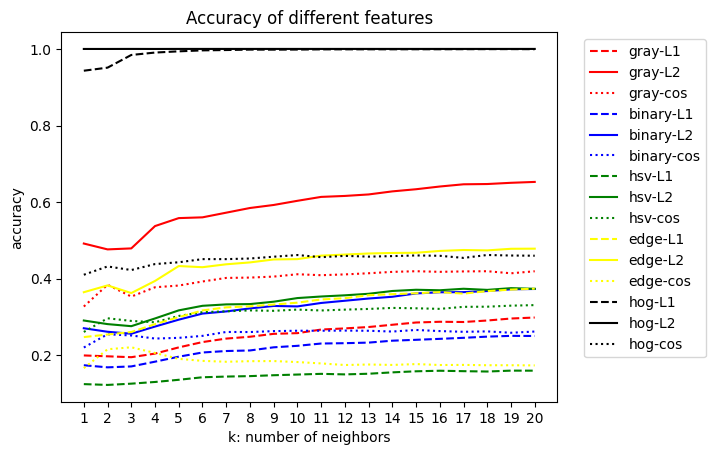
\includegraphics[width=0.5\textwidth]{knn.png}
    \caption{Accuracy of k-NN with different number of neighbors}
    \label{fig:knn}
\end{figure}

\subsection{PCA}
We use cuML to implement the PCA algorithm on GPU, and use the PCA to reduce the dimension of the feature space.
The reslut accuracy of k-NN with PCA with different number of components is shown in Fig 8. From the result, we can see that the accuracy of the classifier will increase as the number of components increases. 
When the number of components is larger than $10$, the accuracy of the classifier will not increase significantly.

\begin{lstlisting}[language=Python, caption={PCA}]
from cuml import PCA

pca = PCA(whiten=True, n_components=1)
pca.fit(train_gray.reshape((50000, -1)).astype(np.float32))
  
train_pca = pca.transform(train_gray.reshape((50000, -1)).astype(np.float32))
test_pca = pca.transform(test_gray.reshape((10000, -1)).astype(np.float32))
\end{lstlisting}

We test the performance of three k-NN classifier with PCA on GPU with different \verb|n_components| from $1$ to $20$, the reslut is shown in Fig 8.
\begin{figure}
    \centering
    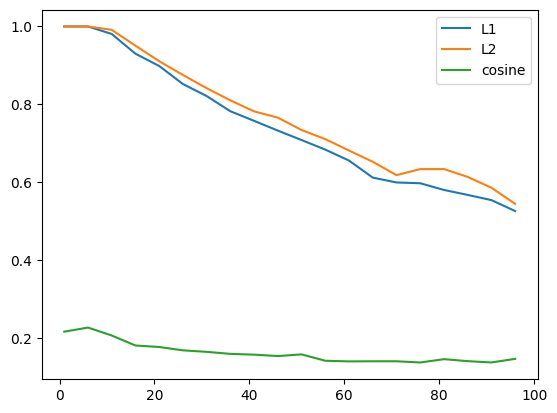
\includegraphics[width=0.5\textwidth]{pca.png}
    \caption{Accuracy of k-NN with PCA with different number of components}
    \label{fig:pca}
\end{figure}

\subsection{SVM}

We use cuML to implement the SVM algorithm on GPU. The reslut accuracy of SVM with different kernel is shown in Fig 9.

The accuracy of SVM classifier is not very high, and the accuracy of Linear SVM with L2 is hightest.
\begin{lstlisting}[language=Python, caption={SVM}]
from cuml import LinearSVC, SVC
classifiers = [
    ('Linear SVM l1', LinearSVC(penalty='l1', loss='squared_hinge', tol=1e-4, C=1.0)),
    ('Linear SVM l2', LinearSVC(penalty='l2', loss='squared_hinge', tol=1e-4, C=1.0)),
    ('SVM rbf', SVC(C=1.0, kernel='rbf', gamma='auto', tol=1e-3)),
    ('SVM sigmoid', SVC(C=1.0, kernel='sigmoid', gamma='auto', tol=1e-3)),
]
\end{lstlisting}
\begin{figure}
    \centering
    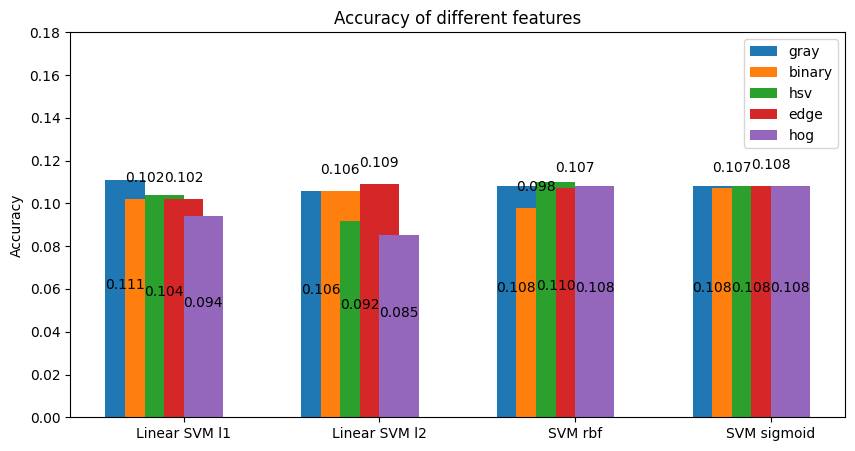
\includegraphics[width=0.5\textwidth]{svm.png}
    \caption{Accuracy of SVM with different kernel}
    \label{fig:svm}
\end{figure}

\section{Conclusion}

In this project, we implement a k-NN classifier to recognize the images in CIFAR-10 dataset. We use different image processing methods to preprocess the dataset, and use different distance metrics to test the performance of the classifier. We also implement a k-NN with PCA classifier, SVM and NN, to compare the performance of the k-NN.

\bibliography{anthology,custom}
\bibliographystyle{acl_natbib}

\end{document}
